\documentclass[aspectratio=169,11pt]{beamer}
\usetheme{Madrid}
\usecolortheme{seahorse}
\setbeamertemplate{navigation symbols}{}
\setbeamertemplate{headline}{}
\setbeamertemplate{footline}[frame number]
\setbeamertemplate{frametitle continuation}{}
\setbeamertemplate{frametitle}{\nointerlineskip\begin{beamercolorbox}[wd=\paperwidth,sep=0.45ex,leftskip=7.5mm,rightskip=7.5mm]{frametitle}\usebeamerfont{frametitle}\insertframetitle\end{beamercolorbox}}
\setbeamerfont{frametitle}{size=\large}
\setbeamerfont{normal text}{size=\normalsize}
\setbeamersize{text margin left=8mm,text margin right=8mm}
\setbeamercolor{keyphrase}{bg=blue!8,fg=black!85}
\setbeameroption{hide notes}
\usepackage{pgfpages}
\pgfpagesuselayout{resize to}[a4paper,landscape]
\usepackage[T1]{fontenc}
\usepackage{tabularx}
\usepackage{array}
\usepackage{booktabs}
\usepackage{listings}
\usepackage{hyperref}
\usepackage{fancyvrb}
\institute{Iwate Prefectural University}
\DeclareUnicodeCharacter{21D2}{\ensuremath{\Rightarrow}}
\DeclareUnicodeCharacter{2227}{\ensuremath{\land}}
\DeclareUnicodeCharacter{00AC}{\ensuremath{\neg}}
\DeclareUnicodeCharacter{2190}{\ensuremath{\leftarrow}}
\lstdefinelanguage{mizar}{morekeywords={definition,end,struct,field,property,inherit,extends,where,from,let,be,being,mode,theorem,proof,thus,hence,by,registration,cluster,coherence,reduce,reducibility,import,for,holds,st,is,func,pred,attribute,algorithm,terminating,requires,ensures,do,while,invariant,decreasing,return,var,const,if,scheme,provided,environ,vocabularies,notations,constructors,registrations,theorems,begin,qua,reconsider,consider,such,that,not,or,and,implies,per,cases,set,thesis},sensitive=true,morecomment=[l]{::}}
\lstdefinelanguage{toml}{morecomment=[l]{\#},morestring=[b]"}
\lstset{basicstyle=\ttfamily\small,keywordstyle=\color{blue!50!black}\bfseries,commentstyle=\color{green!35!black}\itshape,stringstyle=\color{violet!70!black},showstringspaces=false,columns=fullflexible,keepspaces=true,backgroundcolor=\color{black!4},frame=single,rulecolor=\color{black!20},framesep=0.7mm,framerule=0.3pt,xleftmargin=1mm,xrightmargin=1mm,aboveskip=0.6mm,belowskip=0.8mm}
\newcommand{\statusbadge}[2]{\colorbox{#1}{\textcolor{white}{\strut\scriptsize\sffamily\bfseries #2}}}
\newcommand{\badgeMML}{\statusbadge{blue!45!black}{exact MML excerpt}}
\newcommand{\badgeSpec}{\statusbadge{green!35!black}{specification example}}
\newcommand{\badgeSketch}{\statusbadge{orange!75!black}{sketch}}
\newcommand{\deepdivetag}{\hfill\colorbox{black!15}{\textcolor{black!65}{\strut\scriptsize\sffamily deep dive}}}
\pdfstringdefDisableCommands{\def\translate#1{#1}}
\title{Mizar Evo: Design Principles}
\subtitle{Reconnecting automated proof, readable mathematics, and verified computation}
\author{Kazuhisa Nakasho}
\date{{\small\bfseries TPP 2026}\\[1.5mm]{\footnotesize RIKEN AIP Tokyo Office}\\[1mm]{\footnotesize November 16--17, 2026}}

\begin{document}
\begin{frame}
\titlepage
\note{
\smallskip
\textbf{Read aloud:}
\begin{itemize}
\setlength{\itemsep}{1pt}
\setlength{\parsep}{0pt}
\setlength{\parskip}{0pt}
\item \textcolor{blue!55!black}{\textbf{Mizar is a proof checker. It combines first-order set theory, readable mathematical language, and the Mizar Mathematical Library (MML).}}
\item \textcolor{blue!55!black}{\textbf{Mizar Evolution, or Mizar Evo, redesigns the language and its tools. We begin with history and development, then discuss six design principles, implementation limits, and plans.}}
\item Distinguish facts, research hypotheses, and future directions throughout.
\end{itemize}
}
\end{frame}

\section{Part 0. Introduction}
\begin{frame}[fragile,t]{0.2 - Mizar: early systems, Mizar-rs, and Evo}
\par\noindent{\footnotesize\bfseries Table 1. Early Mizar systems and the start of MML\par}
\begin{footnotesize}
\setlength{\tabcolsep}{3pt}
\renewcommand{\arraystretch}{1.15}
\renewcommand{\arraystretch}{0.93}
\begin{tabularx}{\textwidth}{l>{\raggedright\arraybackslash}X}
\toprule
\textbf{Period} & \textbf{Main milestones} \\
\midrule
1973–75 & Mathematical documents → propositional Mizar-PC (Algol / ODRA) \\
1977 & Mizar-QC: quantifiers (Pascal / CDC 6000) \\
1982–84 & MSE: a smaller language. HPF: mathematical notation and implicit arguments \\
1986 & Mizar-4: multiple passes; ported to PC / DOS at the end of the year \\
1988–89 & PC-Mizar, references between articles; MML began on January 1, 1989 \\
\bottomrule
\end{tabularx}
\end{footnotesize}

\par\noindent{\footnotesize\bfseries Table 2. PC-Mizar, Mizar-rs, and Mizar Evo\par}
\begin{footnotesize}
\setlength{\tabcolsep}{3pt}
\renewcommand{\arraystretch}{1.15}
\renewcommand{\arraystretch}{0.93}
\begin{tabularx}{\textwidth}{l>{\raggedright\arraybackslash}X}
\toprule
\textbf{System} & \textbf{Overview} \\
\midrule
PC-Mizar (Pascal) & Parser → MSM → Analyzer → Checker \\
Mizar-rs (Rust, ITP 2023) & Reimplements the checker / analyzer to support the existing language \\
 & \textcolor{blue!55!black}{\textbf{All MML checked:}} replaced the checker; the full MML of that time passed \\
 & \textcolor{blue!55!black}{\textbf{Speed:}} about 5–6× faster (8 threads, elapsed time) \\
 & \textcolor{blue!55!black}{\textbf{Bugs:}} four soundness bugs reported; no false MML proofs used them \\
Mizar Evo (Rust) & New language / processor; keeps mathematical writing and the logical foundation \\
\bottomrule
\end{tabularx}
\end{footnotesize}

{\footnotesize Source: Matuszewski \& Rudnicki (2005); Carneiro (ITP 2023), Table 1.}

\note{
Optional detail (see slide).

\smallskip
\textbf{Optional notes and sources:}
\begin{itemize}
\setlength{\itemsep}{1pt}
\setlength{\parsep}{0pt}
\setlength{\parskip}{0pt}
\item Mizar-PC was propositional; it differs from the later PC-Mizar. Readable notation, checking, and library reuse grew through several experiments and redesigns. These are selected milestones, not a single line of successors. Source details and URLs: \texttt{draft.ja.md}, history and development.
\item Carneiro 2023 §1, footnote 2 dates the PC port to 1986; PC-Mizar dates to 1988. MSM means More Strict Mizar.
\item Mizar-rs elapsed times: checker only, 57.37→11.33 minutes; analyzer plus checker, 71.38→11.71 minutes. Both affect soundness. Compatibility-related issues remain in §5.4 of the paper.
\end{itemize}
\begin{itemize}
\setlength{\itemsep}{1pt}
\setlength{\parsep}{0pt}
\setlength{\parskip}{0pt}
\item {\footnotesize Source: Matuszewski \& Rudnicki (2005); Carneiro (ITP 2023), Table 1.}
\end{itemize}
}
\end{frame}

\begin{frame}[fragile,t]{0.3 - 2023–2026: from an idea to language design}
\par\noindent{\footnotesize\bfseries Table 3. Mizar Evo development\par}
\begin{footnotesize}
\setlength{\tabcolsep}{3pt}
\renewcommand{\arraystretch}{1.15}
\begin{tabularx}{\textwidth}{l>{\raggedright\arraybackslash}X}
\toprule
\textbf{Period} & \textbf{Development} \\
\midrule
Aug 2023 & First README: mizar-wishlist \\
Sep–Oct 2024 & Imports, namespaces, structure inheritance, type system \\
May–Jun 2025 & Modes, inference, redefinition; dependent structures / attributes removed and restored \\
Jan–Apr 2026 & EBNF, logical encoding, registration, template and algorithm semantics / contracts \\
May 2026 & Implementation design → test harness → minimal lexer \\
\bottomrule
\end{tabularx}
\end{footnotesize}

\begin{itemize}
\setlength{\itemsep}{1pt}
\setlength{\parsep}{0pt}
\setlength{\parskip}{0pt}
\item \textcolor{blue!55!black}{\textbf{Preparing the 2023 grant proposal changed the plan: from notation extensions to a new language and processor.}}
\item ITP 2023: Mario Carneiro welcomed a request for implementation help. CICM 2023: wishlist discussion with Adam Naumowicz.
\item Early priorities: generic types, namespaces / packages, ATP / traceability. The prototype was to use Mizar-rs.
\end{itemize}
{\footnotesize JSPS KAKENHI, Scientific Research (C), awarded in 2024: 24K14897, “Renewing the language specification of a set-theory-based proof assistant” (title translated).}

\note{
\smallskip
\textbf{Read aloud:}
\begin{itemize}
\setlength{\itemsep}{1pt}
\setlength{\parsep}{0pt}
\setlength{\parskip}{0pt}
\item \textcolor{blue!55!black}{\textbf{Preparing the 2023 grant proposal changed the plan: from notation extensions to a new language and processor.}}
\item ITP 2023: Mario Carneiro welcomed a request for implementation help. CICM 2023: wishlist discussion with Adam Naumowicz.
\item Early priorities: generic types, namespaces / packages, ATP / traceability. The prototype was to use Mizar-rs.
\item {\footnotesize JSPS KAKENHI, Scientific Research (C), awarded in 2024: 24K14897, “Renewing the language specification of a set-theory-based proof assistant” (title translated).}
\end{itemize}
\smallskip
\textbf{Optional notes and sources:}
\begin{itemize}
\setlength{\itemsep}{1pt}
\setlength{\parsep}{0pt}
\setlength{\parskip}{0pt}
\item Source: August 2023 grant proposal and Git diffs. Details: \texttt{draft.ja.md}, history and development.
\item The exact order of the consultations within 2023 and any current participation commitment are unconfirmed. Timeline dates are commit dates.
\end{itemize}
}
\end{frame}

\begin{frame}[fragile,t]{0.4 - Design development and implementation with AI agents}
\smallskip
\textbf{Developing the language design}
\begin{itemize}
\setlength{\itemsep}{1pt}
\setlength{\parsep}{0pt}
\setlength{\parskip}{0pt}
\item \textcolor{blue!55!black}{\textbf{template:}} from generics to a common theorem form for schemes, with structure views and type-argument inference.
\item \textcolor{blue!55!black}{\textbf{algorithm:}} early requests from Japanese Mizar cryptographers for algorithm proofs, and difficult symbolic calculations in elliptic-curve associativity.
\end{itemize}
\smallskip
\textbf{Implementation and discussions since May 2026}
\begin{itemize}
\setlength{\itemsep}{1pt}
\setlength{\parsep}{0pt}
\setlength{\parskip}{0pt}
\item \textcolor{blue!55!black}{\textbf{May: began Rust implementation with AI coding agents. June–July: crate development, agent workflows, SAT-backed checking and audits.}}
\item \textcolor{blue!55!black}{\textbf{Design → agent implementation → tests and audits → specification revision.}}
\item September: seminar and discussions with the Mizar team in Bia\l{}ystok.
\item September–October: more proof obligations from source; changes to algorithm partiality and contracts.
\end{itemize}
\note{
\smallskip
\textbf{Read aloud:}
\begin{itemize}
\setlength{\itemsep}{1pt}
\setlength{\parsep}{0pt}
\setlength{\parskip}{0pt}
\item \textcolor{blue!55!black}{\textbf{template:}} from generics to a common theorem form for schemes, with structure views and type-argument inference.
\item \textcolor{blue!55!black}{\textbf{algorithm:}} early requests from Japanese Mizar cryptographers for algorithm proofs, and difficult symbolic calculations in elliptic-curve associativity.
\item \textcolor{blue!55!black}{\textbf{May: began Rust implementation with AI coding agents. June–July: crate development, agent workflows, SAT-backed checking and audits.}}
\item \textcolor{blue!55!black}{\textbf{Design → agent implementation → tests and audits → specification revision.}}
\item September: seminar and discussions with the Mizar team in Bia\l{}ystok.
\item September–October: more proof obligations from source; changes to algorithm partiality and contracts.
\end{itemize}
\smallskip
\textbf{Optional notes and sources:}
\begin{itemize}
\setlength{\itemsep}{1pt}
\setlength{\parsep}{0pt}
\setlength{\parskip}{0pt}
\item Source: spec 18/20, Git diffs, author's account (2026-10-15); \texttt{draft.ja.md}.
\end{itemize}
}
\end{frame}

\begin{frame}[fragile,t]{0.5 - Six challenges and design principles}
\par\noindent{\footnotesize\bfseries Table 4. Six challenges and design principles\par}
\begin{small}
\setlength{\tabcolsep}{3pt}
\renewcommand{\arraystretch}{1.35}
\begin{tabularx}{\textwidth}{l>{\raggedright\arraybackslash}X>{\raggedright\arraybackslash}X}
\toprule
\textbf{Area} & \textbf{Challenge in current Mizar} & \textbf{Design principle} \\
\midrule
\textcolor{blue!55!black}{\textbf{§1 Foundation}} & Keep the logic and MML while replacing the processor & Keep FOL / set theory and a small kernel \\
\textcolor{blue!55!black}{\textbf{§2 Writing}} & Trace implicit type, registration, and overload choices & Keep mathematical abstractions; explain implicit choices \\
\textcolor{blue!55!black}{\textbf{§3 Generics}} & Separate mechanisms for definitions, theorems, and schemes & Unify generic mechanisms with templates \\
\textcolor{blue!55!black}{\textbf{§4 Computation}} & Connect proofs to executable procedures & Check algorithm contracts, invariants, and termination \\
\textcolor{blue!55!black}{\textbf{§5 Tools}} & Dependencies, distribution, incremental checking, IDE & Modules, namespaces, packages, incremental builds, LSP \\
\textcolor{blue!55!black}{\textbf{§6 Checking}} & Connect external search to checking evidence & Use ATPs; instantiate evidence and check with SAT \\
\bottomrule
\end{tabularx}
\end{small}

\note{
Optional detail (see slide).

\smallskip
\textbf{Optional notes and sources:}
\begin{itemize}
\setlength{\itemsep}{1pt}
\setlength{\parsep}{0pt}
\setlength{\parskip}{0pt}
\item Each row connects a challenge to a principle; sections 1–6 follow this order. First-order foundations and readable mathematics are strengths to preserve.
\item The closing status section distinguishes the specification from implemented behavior.
\item Source: specification chapters 01, 18, 20, 21, 23; the problem-driven stories in the Bia\l{}ystok deck.
\end{itemize}
}
\end{frame}

\section{Part 1. Logical Foundation}
\begin{frame}[fragile,t]{1.1 - Keep the foundation, rebuild the tools}
\begin{center}
\begin{beamercolorbox}[rounded=true,sep=2.5mm,wd=0.9\textwidth]{keyphrase}
\centering\itshape \textcolor{blue!55!black}{\textbf{Keep the mathematical language.}}\\ \textcolor{blue!55!black}{\textbf{Rebuild the processor and development tools.}}
\end{beamercolorbox}
\end{center}
\begin{itemize}
\setlength{\itemsep}{1pt}
\setlength{\parsep}{0pt}
\setlength{\parskip}{0pt}
\item \textcolor{blue!55!black}{\textbf{Keep first-order logic (FOL) and Tarski–Grothendieck set theory.}}
\item Keep soft types, modes, attributes, registrations, structures, and declarative proofs.
\item \textcolor{blue!55!black}{\textbf{Separate ATP search from checking: a small kernel independently checks the results. Details in §6.}}
\end{itemize}
\note{
\smallskip
\textbf{Read aloud:}
\begin{itemize}
\setlength{\itemsep}{1pt}
\setlength{\parsep}{0pt}
\setlength{\parskip}{0pt}
\item \textcolor{blue!55!black}{\textbf{Keep the mathematical language.}} \textcolor{blue!55!black}{\textbf{Rebuild the processor and development tools.}}
\item \textcolor{blue!55!black}{\textbf{Keep first-order logic (FOL) and Tarski–Grothendieck set theory.}}
\item Keep soft types, modes, attributes, registrations, structures, and declarative proofs.
\item \textcolor{blue!55!black}{\textbf{Separate ATP search from checking: a small kernel independently checks the results. Details in §6.}}
\end{itemize}
\smallskip
\textbf{Optional notes and sources:}
\begin{itemize}
\setlength{\itemsep}{1pt}
\setlength{\parsep}{0pt}
\setlength{\parskip}{0pt}
\item Mathematical language and proof support can be built over a first-order foundation. Similar mechanisms do not imply identical logics or representations.
\item Success rates and reconstruction failures do not establish a first-order performance advantage. Evaluate the design through mathematical writing, automation, and proof checking.
\end{itemize}
}
\end{frame}

\begin{frame}[fragile,t]{1.2 - From sets to topological spaces}
\smallskip
\textbf{Example 1: Cantor's theorem in current Mizar}~\badgeSketch~{\footnotesize(proof omitted)}
\begin{lstlisting}[language={mizar},basicstyle=\ttfamily\small]
theorem Cantor:
  for X being set holds card X in card (bool X)
proof ... end;
\end{lstlisting}
Example 2: a continuous bijection from a compact space to a Hausdorff space (sketch, proof omitted):

\begin{lstlisting}[language={mizar},basicstyle=\ttfamily\small]
theorem CompactBijection:
  for S being compact TopSpace,
      T being non empty T_2 TopSpace,
      f being Function of S,T
  st f is continuous one-to-one & rng f = [#] T
  holds f is being_homeomorphism
proof ... end;
\end{lstlisting}
\begin{itemize}
\setlength{\itemsep}{1pt}
\setlength{\parsep}{0pt}
\setlength{\parskip}{0pt}
\item \textcolor{blue!55!black}{\textbf{Write mathematics from sets, power sets, and cardinals to topological spaces over first-order set theory.}}
\end{itemize}
\note{
\smallskip
\textbf{Read aloud:}
\begin{itemize}
\setlength{\itemsep}{1pt}
\setlength{\parsep}{0pt}
\setlength{\parskip}{0pt}
\item Example 1: Cantor's theorem in current Mizar.
\item Example 2: a continuous bijection from a compact space to a Hausdorff space.
\item \textcolor{blue!55!black}{\textbf{Write mathematics from sets, power sets, and cardinals to topological spaces over first-order set theory.}}
\end{itemize}
\smallskip
\textbf{Optional notes and sources:}
\begin{itemize}
\setlength{\itemsep}{1pt}
\setlength{\parsep}{0pt}
\setlength{\parskip}{0pt}
\item Source: CARD\_1:14 and COMPTS\_1:17 (\texttt{draft.ja.md} §1). Spend about 30 seconds on each example, pointing out the meaning and language features. Proofs are omitted; these are explanatory sketches, not execution results.
\item Cantor: bool X is the power set. Cardinals are initial ordinals, so in expresses a strict cardinal inequality here. Topology: T\_2 means Hausdorff; rng f = [\#] T means surjective; the conclusion states that f is a homeomorphism. Search and checking are separated in §6.
\end{itemize}
}
\end{frame}

\section{Part 2. Readable Mathematics}
\begin{frame}[fragile,t]{2.1 - Trace type, registration, and overload choices}
Readable mathematics relies on many automatic decisions.

\begin{itemize}
\setlength{\itemsep}{1pt}
\setlength{\parsep}{0pt}
\setlength{\parskip}{0pt}
\item \textcolor{blue!55!black}{\textbf{type: which types can this object be used as?}} Follow attributes and inheritance. Example: Group → Magma, with a unique path.
\item \textcolor{blue!55!black}{\textbf{registration: which rules supplied the required attributes?}} Example: the chain empty → finite → countable.
\item \textcolor{blue!55!black}{\textbf{overload: which definition and view were selected?}} Distinguish definitions with the same notation, or addition and multiplication in a ring.
\end{itemize}
\textcolor{blue!55!black}{\textbf{Keep natural writing and automatic rules, while tracing the reasons for implicit choices.}}

\note{
\smallskip
\textbf{Read aloud:}
\begin{itemize}
\setlength{\itemsep}{1pt}
\setlength{\parsep}{0pt}
\setlength{\parskip}{0pt}
\item Readable mathematics relies on many automatic decisions.
\item \textcolor{blue!55!black}{\textbf{type: which types can this object be used as?}} Follow attributes and inheritance. Example: Group → Magma, with a unique path.
\item \textcolor{blue!55!black}{\textbf{registration: which rules supplied the required attributes?}} Example: the chain empty → finite → countable.
\item \textcolor{blue!55!black}{\textbf{overload: which definition and view were selected?}} Distinguish definitions with the same notation, or addition and multiplication in a ring.
\item \textcolor{blue!55!black}{\textbf{Keep natural writing and automatic rules, while tracing the reasons for implicit choices.}}
\end{itemize}
\smallskip
\textbf{Optional notes and sources:}
\begin{itemize}
\setlength{\itemsep}{1pt}
\setlength{\parsep}{0pt}
\setlength{\parskip}{0pt}
\item Source: spec 08 §8.1–8.2; 17 §17.7; 19 §19.1–19.3. Type: 2.2–2.4; registration: 2.5; overload / views: 2.6.
\end{itemize}
}
\end{frame}

\begin{frame}[fragile,t]{2.2 - type: declare fields and properties}
\smallskip
\textbf{Structure declarations}~\badgeSpec~{\footnotesize(inside a definition block)}
\begin{lstlisting}[language={mizar},basicstyle=\ttfamily\footnotesize]
struct LoopStr where
  field carrier -> set;
  field binop -> BinOp of carrier;
  property unit -> Element of carrier;
end;

struct AddLoopStr where
  field carrier -> set;
  field add -> BinOp of carrier;
  property zero -> Element of carrier;
end;
\end{lstlisting}
\textcolor{blue!55!black}{\textbf{A field stores data. A property declares a name and type; its implementation is given separately.}}

\note{
\smallskip
\textbf{Read aloud:}
\begin{itemize}
\setlength{\itemsep}{1pt}
\setlength{\parsep}{0pt}
\setlength{\parskip}{0pt}
\item Structure declarations.
\item \textcolor{blue!55!black}{\textbf{A field stores data. A property declares a name and type; its implementation is given separately.}}
\end{itemize}
\smallskip
\textbf{Optional notes and sources:}
\begin{itemize}
\setlength{\itemsep}{1pt}
\setlength{\parsep}{0pt}
\setlength{\parskip}{0pt}
\item Source: \texttt{doc/spec/en/05.structures.md} §5.2, 5.5.1; \texttt{sample\_codes.md}, LoopStr and AddLoopStr. These declarations are excerpts inside a definition block. Only fields are constructor arguments. Inheritance follows in 2.3, then the mode and unit implementation in 2.4.
\end{itemize}
}
\end{frame}

\begin{frame}[fragile,t]{2.3 - type: declare inheritance after the structure}
\smallskip
\textbf{Add a parent mapping after declaring AddLoopStr}~\badgeSpec
\begin{lstlisting}[language={mizar},basicstyle=\ttfamily\small]
definition
  inherit AddLoopStr extends LoopStr where
    field carrier from carrier;
    field add from binop;
    property zero from unit;
  end;
end;
\end{lstlisting}
\begin{itemize}
\setlength{\itemsep}{1pt}
\setlength{\parsep}{0pt}
\setlength{\parskip}{0pt}
\item \textcolor{blue!55!black}{\textbf{Separate structure declarations from inheritance. This is similar to implementing a Rust trait after defining a type.}}
\item \texttt{from} renames a parent's role: \texttt{binop} becomes \texttt{add}, and \texttt{unit} becomes \texttt{zero}.
\item One declaration per parent. Equal member types need no proof; narrower types require \texttt{coherence}.
\end{itemize}
\note{
\smallskip
\textbf{Read aloud:}
\begin{itemize}
\setlength{\itemsep}{1pt}
\setlength{\parsep}{0pt}
\setlength{\parskip}{0pt}
\item Add a parent mapping after declaring AddLoopStr.
\item \textcolor{blue!55!black}{\textbf{Separate structure declarations from inheritance. This is similar to implementing a Rust trait after defining a type.}}
\item \texttt{from} renames a parent's role: \texttt{binop} becomes \texttt{add}, and \texttt{unit} becomes \texttt{zero}.
\item One declaration per parent. Equal member types need no proof; narrower types require \texttt{coherence}.
\end{itemize}
\smallskip
\textbf{Optional notes and sources:}
\begin{itemize}
\setlength{\itemsep}{1pt}
\setlength{\parsep}{0pt}
\setlength{\parskip}{0pt}
\item Source: \texttt{doc/spec/en/05.structures.md} §5.3; \texttt{sample\_codes.md}, AddLoopStr. The Rust analogy concerns the separation of declarations. In LoopStr, binop is a field and unit is a property.
\end{itemize}
}
\end{frame}

\begin{frame}[fragile,t]{2.4 - type: implement unit for Unital, reuse it as zero}
has\_unit states that a two-sided identity exists; it does not depend on unit (sketch):

\begin{lstlisting}[language={mizar},basicstyle=\ttfamily\footnotesize]
definition
  mode UnitalDef: Unital is has_unit LoopStr;
  let M be Unital;
  property M.unit means
    for x being Element of M.carrier holds
      M.binop(it,x) = x & M.binop(x,it) = x;
  existence proof ... end;
  uniqueness proof ... end;
end;
\end{lstlisting}
\begin{itemize}
\setlength{\itemsep}{1pt}
\setlength{\parsep}{0pt}
\setlength{\parskip}{0pt}
\item \textcolor{blue!55!black}{\textbf{If A's selected LoopStr view is Unital, reuse its unit implementation as zero.}}
\item \texttt{property zero from unit} gives \texttt{A.zero = (A qua LoopStr).unit}. No new zero implementation is needed.
\end{itemize}
\note{
\smallskip
\textbf{Read aloud:}
\begin{itemize}
\setlength{\itemsep}{1pt}
\setlength{\parsep}{0pt}
\setlength{\parskip}{0pt}
\item has\_unit states that a two-sided identity exists; it does not depend on unit.
\item \textcolor{blue!55!black}{\textbf{If A's selected LoopStr view is Unital, reuse its unit implementation as zero.}}
\item \texttt{property zero from unit} gives \texttt{A.zero = (A qua LoopStr).unit}. No new zero implementation is needed.
\end{itemize}
\smallskip
\textbf{Optional notes and sources:}
\begin{itemize}
\setlength{\itemsep}{1pt}
\setlength{\parsep}{0pt}
\setlength{\parskip}{0pt}
\item Source: \texttt{doc/spec/en/07.modes.md} §7.4.1, 7.8.2; \texttt{05.structures.md} §5.3, 5.8.3. Sketch adapting the implementation example in chapter 7 to LoopStr. The has\_unit definition is in \texttt{draft.ja.md}; proof bodies are omitted. Existence follows from the mode assumption, uniqueness by applying the operation to two identities.
\item A is AddLoopStr, and the selected LoopStr view must satisfy Unital. Do not mix facts from different views. This example has no overlapping implementations; overlaps require coherence.
\end{itemize}
}
\end{frame}

\begin{frame}[fragile,t]{2.5 - registration: automatic chains hide dependencies}
\textcolor{blue!55!black}{\textbf{Automatic rule chains hide dependencies at the point of use.}}

\begin{lstlisting}[language={mizar},basicstyle=\ttfamily\small]
registration
  cluster EmptyImpliesFinite: empty -> finite for set;
  coherence proof ... end;
  cluster FiniteImpliesCountable: finite -> countable for set;
  coherence proof ... end;
end;
\end{lstlisting}
\par\noindent{\footnotesize\bfseries Table 5. Registration paths recorded by the new specification\par}
\begin{footnotesize}
\setlength{\tabcolsep}{3pt}
\renewcommand{\arraystretch}{1.15}
\begin{tabular}{lll}
\toprule
\textbf{Starting fact} & \textbf{Derived fact} & \textbf{Recorded rule} \\
\midrule
S is empty & S is finite & EmptyImpliesFinite \\
S is finite & S is countable & FiniteImpliesCountable \\
\bottomrule
\end{tabular}
\end{footnotesize}

\begin{itemize}
\setlength{\itemsep}{1pt}
\setlength{\parsep}{0pt}
\setlength{\parskip}{0pt}
\item Declaring \texttt{empty} gives \texttt{finite} and then \texttt{countable} implicitly. No rule citation with \texttt{by} is needed.
\item \textcolor{blue!55!black}{\textbf{New specification: keep automatic application, and record rule labels and application paths.}}
\end{itemize}
\note{
\smallskip
\textbf{Read aloud:}
\begin{itemize}
\setlength{\itemsep}{1pt}
\setlength{\parsep}{0pt}
\setlength{\parskip}{0pt}
\item \textcolor{blue!55!black}{\textbf{Automatic rule chains hide dependencies at the point of use.}}
\item Declaring \texttt{empty} gives \texttt{finite} and then \texttt{countable} implicitly. No rule citation with \texttt{by} is needed.
\item \textcolor{blue!55!black}{\textbf{New specification: keep automatic application, and record rule labels and application paths.}}
\end{itemize}
\smallskip
\textbf{Optional notes and sources:}
\begin{itemize}
\setlength{\itemsep}{1pt}
\setlength{\parsep}{0pt}
\setlength{\parskip}{0pt}
\item Source: \texttt{doc/spec/en/17.clusters\_and\_registrations.md} §17.2, 17.4.1, 17.7; \texttt{23.package\_management\_and\_build\_system.md} §23.7.7. Labeled registration example from the new specification; the table is an explanatory trace for an empty set S.
\item Emphasize that rules are not cited at the point of use and can apply in several stages. Attribute resolution takes place before ATP search.
\end{itemize}
}
\end{frame}

\begin{frame}[fragile,t]{2.6 - overload: two identities in the same ring}
\textcolor{blue!55!black}{\textbf{In the same ring R, the additive identity is 0 and the multiplicative identity is 1.}}

\begin{itemize}
\setlength{\itemsep}{1pt}
\setlength{\parsep}{0pt}
\setlength{\parskip}{0pt}
\item Additive AddMagma: \texttt{0 + x = x + 0 = x}
\item Multiplicative MulMagma: \texttt{1 * x = x * 1 = x}
\end{itemize}
\smallskip
\textbf{id. M returns the identity of a unital Magma M}~\badgeSketch~{\footnotesize(definition omitted)}
\begin{lstlisting}[language={mizar},basicstyle=\ttfamily\small]
let R be Ring;
id. R;                   :: ambiguous Magma view
id. (R qua AddMagma);     :: R.zero
id. (R qua MulMagma);     :: R.one
\end{lstlisting}
\begin{itemize}
\setlength{\itemsep}{1pt}
\setlength{\parsep}{0pt}
\setlength{\parskip}{0pt}
\item Even with one definition of id., the Magma view of R is ambiguous.
\item \textcolor{blue!55!black}{\textbf{Use qua to select the additive or multiplicative view and distinguish 0 from 1.}}
\end{itemize}
\note{
\smallskip
\textbf{Read aloud:}
\begin{itemize}
\setlength{\itemsep}{1pt}
\setlength{\parsep}{0pt}
\setlength{\parskip}{0pt}
\item \textcolor{blue!55!black}{\textbf{In the same ring R, the additive identity is 0 and the multiplicative identity is 1.}}
\item Additive AddMagma: \texttt{0 + x = x + 0 = x}
\item Multiplicative MulMagma: \texttt{1 * x = x * 1 = x}
\item id. M returns the identity of a unital Magma M.
\item Even with one definition of id., the Magma view of R is ambiguous.
\item \textcolor{blue!55!black}{\textbf{Use qua to select the additive or multiplicative view and distinguish 0 from 1.}}
\end{itemize}
\smallskip
\textbf{Optional notes and sources:}
\begin{itemize}
\setlength{\itemsep}{1pt}
\setlength{\parsep}{0pt}
\setlength{\parskip}{0pt}
\item Source: \texttt{doc/spec/en/sample\_codes.md}, IdentityDef, LoopUnitalDef, RingLikeDef; \texttt{19.overload\_resolution.md} §19.2.2–19.3.1; \texttt{05.structures.md} §5.8.3.
\item Sketch limited to the identity functor id. Assume both views are unital, their identities correspond to R.zero / R.one, and each path to Magma is unique. Definitions: \texttt{draft.ja.md}.
\end{itemize}
}
\end{frame}

\section{Part 3. Generic Mathematics}
\begin{frame}[fragile,t]{3.1 - Current MML: more types, more redefinitions and registrations}
\textcolor{blue!55!black}{\textbf{The sum of functions has one body, but preserving result types needs work for each type.}}

\par\noindent{\footnotesize\bfseries Table 6. Per-type declarations for function addition in VALUED\_1\par}
\begin{scriptsize}
\setlength{\tabcolsep}{3pt}
\renewcommand{\arraystretch}{1.15}
\begin{tabular}{lll}
\toprule
\textbf{Value type} & \textbf{Result-type redefinition} & \textbf{Attribute / totality registration} \\
\midrule
Complex & \texttt{PartFunc of C,COMPLEX} & \texttt{complex-valued} + \texttt{total} \\
Real & \texttt{PartFunc of C,REAL} & \texttt{real-valued} + \texttt{total} \\
Rational & \texttt{PartFunc of C,RAT} & \texttt{RAT-valued} + \texttt{total} \\
Integer & \texttt{PartFunc of C,INT} & \texttt{INT-valued} + \texttt{total} \\
Natural & \texttt{PartFunc of C,NAT} & \texttt{natural-valued} + \texttt{total} \\
\bottomrule
\end{tabular}
\end{scriptsize}

\begin{itemize}
\setlength{\itemsep}{1pt}
\setlength{\parsep}{0pt}
\setlength{\parskip}{0pt}
\item \textcolor{blue!55!black}{\textbf{Each new type adds redefinitions, registrations, and coherence proofs.}}
\item We want one template for function addition and its result type.
\end{itemize}
\note{
\smallskip
\textbf{Read aloud:}
\begin{itemize}
\setlength{\itemsep}{1pt}
\setlength{\parsep}{0pt}
\setlength{\parskip}{0pt}
\item \textcolor{blue!55!black}{\textbf{The sum of functions has one body, but preserving result types needs work for each type.}}
\item \textcolor{blue!55!black}{\textbf{Each new type adds redefinitions, registrations, and coherence proofs.}}
\item We want one template for function addition and its result type.
\end{itemize}
\smallskip
\textbf{Optional notes and sources:}
\begin{itemize}
\setlength{\itemsep}{1pt}
\setlength{\parsep}{0pt}
\setlength{\parskip}{0pt}
\item Source: MML VALUED\_1 (\url{https://mizar.uwb.edu.pl/version/current/html/valued\_1.html}), def 1 and five following groups of attribute / total registrations and PartFunc redefinitions. Table summary, not a quotation. C is the common domain. Each row assumes its input value type; total registration also needs total inputs and nonempty ranges. All redefinitions / registrations have coherence proofs.
\item The body of VALUED\_1:def 1 is shared and uses the intersection of domains. The next template sketch is restricted to a common nonempty domain I.
\end{itemize}
}
\end{frame}

\begin{frame}[fragile,t]{3.2 - template: share the body and result type}
\smallskip
\textbf{Generic functor}~\badgeSketch~{\footnotesize(existence and uniqueness proofs omitted)}
\begin{lstlisting}[language={mizar},basicstyle=\ttfamily\footnotesize]
definition
  let T be type extends non empty AddMagma;
  let I be non empty set;
  let f, g be Function of I, T.carrier;
  func AddDef: Add[T,I](f,g) -> Function of I,T.carrier means
    for i being Element of I holds it.i = T.add(f.i,g.i);
  synonym f +[T,I] g for Add[T,I](f,g);
end;
\end{lstlisting}
\par\noindent{\footnotesize\bfseries Table 7. Template instances and result types\par}
\begin{footnotesize}
\setlength{\tabcolsep}{3pt}
\renewcommand{\arraystretch}{1.15}
\begin{tabularx}{\textwidth}{l>{\raggedright\arraybackslash}X}
\toprule
\textbf{Call (real R / complex C)\footnotemark[1]} & \textbf{Result type} \\
\midrule
\texttt{f + g} & \texttt{Function of I,R.carrier} \\
\texttt{u + v} & \texttt{Function of I,C.carrier} \\
\bottomrule
\end{tabularx}
\end{footnotesize}

\begin{itemize}
\setlength{\itemsep}{1pt}
\setlength{\parsep}{0pt}
\setlength{\parskip}{0pt}
\item \textcolor{blue!55!black}{\textbf{One definition gives the sum and its result type for each number system.}}
\end{itemize}
\footnotetext[1]{Explicit forms: \texttt{f +[R,I] g}, \texttt{u +[C,I] v}. Omit arguments only when declared types determine them uniquely. Use \texttt{qua} for ambiguous inheritance paths.}
\note{
\smallskip
\textbf{Read aloud:}
\begin{itemize}
\setlength{\itemsep}{1pt}
\setlength{\parsep}{0pt}
\setlength{\parskip}{0pt}
\item Generic functor.
\item \textcolor{blue!55!black}{\textbf{One definition gives the sum and its result type for each number system.}}
\end{itemize}
\smallskip
\textbf{Optional notes and sources:}
\begin{itemize}
\setlength{\itemsep}{1pt}
\setlength{\parsep}{0pt}
\setlength{\parskip}{0pt}
\item Assume RealAdd R, ComplexAdd C, and required registrations, with unique paths to non empty AddMagma. f,g: Function of I,R.carrier; u,v: Function of I,C.carrier. Declared types uniquely determine T,I. Other number types need additive structures, closure, registrations. synonym supplies +.
\item Source: spec 11 §11.1.2; 18 §18.2.2, 18.2.7, 18.7; 19 §19.6.2. A range set alone does not select addition; qua views are not inferred.
\end{itemize}
\begin{itemize}
\setlength{\itemsep}{1pt}
\setlength{\parsep}{0pt}
\setlength{\parskip}{0pt}
\item Explicit forms: \texttt{f +[R,I] g}, \texttt{u +[C,I] v}. Omit arguments only when declared types determine them uniquely. Use \texttt{qua} for ambiguous inheritance paths.
\end{itemize}
}
\end{frame}

\begin{frame}[fragile,t]{3.3 - Unify schemes with template theorems\deepdivetag}
\smallskip
\textbf{Induction as a theorem with a predicate parameter}~\badgeSpec
\begin{lstlisting}[language={mizar},basicstyle=\ttfamily\small]
definition
  let P be pred(Nat);
  theorem NatInduction[P]:
    P(0) & (for n being Nat st P(n) holds P(n+1))
    implies for n being Nat holds P(n)
  proof ... end;
end;
\end{lstlisting}
\begin{itemize}
\setlength{\itemsep}{1pt}
\setlength{\parsep}{0pt}
\setlength{\parskip}{0pt}
\item A predicate parameter describes a family of first-order theorems, one per substituted predicate.\footnotemark[1]
\item Explicit instantiation: \texttt{defpred}, followed by \texttt{by NatInduction[P], Base, Step}.
\item Functor parameters are schema-level symbols, not sets. The logic stays first-order.
\end{itemize}
\footnotetext[1]{Details: Bia\l{}ystok deck, Story 6 (\texttt{PermProduct[T]} and views with \texttt{qua}); also Backup 1 here.}
\note{
\smallskip
\textbf{Read aloud:}
\begin{itemize}
\setlength{\itemsep}{1pt}
\setlength{\parsep}{0pt}
\setlength{\parskip}{0pt}
\item Induction as a theorem with a predicate parameter.
\item A predicate parameter describes a family of first-order theorems, one per substituted predicate.\footnotemark[1]
\item Explicit instantiation: \texttt{defpred}, followed by \texttt{by NatInduction[P], Base, Step}.
\item Functor parameters are schema-level symbols, not sets. The logic stays first-order.
\end{itemize}
\smallskip
\textbf{Optional notes and sources:}
\begin{itemize}
\setlength{\itemsep}{1pt}
\setlength{\parsep}{0pt}
\setlength{\parskip}{0pt}
\item Source: \texttt{doc/spec/en/18.templates.md} §18.2.3, 18.8.2, 18.9. Frame 3.4 shows type / value parameters for structures and attributes.
\end{itemize}
\begin{itemize}
\setlength{\itemsep}{1pt}
\setlength{\parsep}{0pt}
\setlength{\parskip}{0pt}
\item Details: Bia\l{}ystok deck, Story 6 (\texttt{PermProduct[T]} and views with \texttt{qua}); also Backup 1 here.
\end{itemize}
}
\end{frame}

\begin{frame}[fragile,t]{3.4 - template: parameterize structures and attributes too}
\smallskip
\textbf{struct: vector-space data over a field K}~\badgeSketch~{\footnotesize(inside a definition block)}
\begin{lstlisting}[language={mizar},basicstyle=\ttfamily\small]
let K be Field;
struct VectorSpace[K] where
  field carrier -> non empty set;
  field add -> BinOp of carrier;
  field smul -> Function of [:K.carrier, carrier:], carrier;
end;
\end{lstlisting}
\texttt{of} / \texttt{over} are syntactic sugar (shorter notation): \texttt{Vector of K} → \texttt{Vector[K]} (a mode example).

\smallskip
\textbf{attr: a subset S is dense in a space M}~\badgeSketch~{\footnotesize(condition omitted)}
\begin{lstlisting}[language={mizar},basicstyle=\ttfamily\small]
let M be MetricSpace;
let S be Subset of M.carrier;
attr DenseDef: S is dense[M] means ...;
\end{lstlisting}
Prefix attributes are also syntactic sugar: \texttt{M-dense} → \texttt{dense[M]}.

\textcolor{blue!55!black}{\textbf{Type / value parameters are shared across struct, attr, mode, pred, and func.}}

\note{
\smallskip
\textbf{Read aloud:}
\begin{itemize}
\setlength{\itemsep}{1pt}
\setlength{\parsep}{0pt}
\setlength{\parskip}{0pt}
\item struct: vector-space data over a field K.
\item \texttt{of} / \texttt{over} are syntactic sugar (shorter notation): \texttt{Vector of K} → \texttt{Vector[K]} (a mode example).
\item attr: a subset S is dense in a space M.
\item Prefix attributes are also syntactic sugar: \texttt{M-dense} → \texttt{dense[M]}.
\item \textcolor{blue!55!black}{\textbf{Type / value parameters are shared across struct, attr, mode, pred, and func.}}
\end{itemize}
\smallskip
\textbf{Optional notes and sources:}
\begin{itemize}
\setlength{\itemsep}{1pt}
\setlength{\parsep}{0pt}
\setlength{\parskip}{0pt}
\item Source: \texttt{doc/spec/en/18.templates.md} §18.1, 18.2.6, 18.3, 18.5. Excerpts inside a definition block; vector-space laws and the density condition are omitted. Assume a mode Vector taking K and its of synonym. VectorSpace over K is also a synonym for VectorSpace[K]. Predicate / functor parameters are restricted to theorem and algorithm.
\item In the 35-minute version, spend 15 seconds pointing to structure and attribute parameters.
\end{itemize}
}
\end{frame}

\section{Part 4. Verified Computation}
\begin{frame}[fragile,t]{4.1 - Computation: verified algorithms}
\textcolor{blue!55!black}{\textbf{Apply Hoare rules recursively to generate first-order proof obligations:}}

\begin{center}
\begin{beamercolorbox}[rounded=true,sep=2.5mm,wd=0.9\textwidth]{keyphrase}
\centering\itshape \{ requires \}  algorithm body  \{ ensures \}
\end{beamercolorbox}
\end{center}
P / Q: precondition / postcondition; B: condition; I: invariant; S: statement.

\par\noindent{\footnotesize\bfseries Table 8. Basic Hoare rules\par}
\begin{footnotesize}
\setlength{\tabcolsep}{3pt}
\renewcommand{\arraystretch}{1.15}
\begin{tabularx}{\textwidth}{l>{\raggedright\arraybackslash}X}
\toprule
\textbf{Syntax} & \textbf{Conditions to check (partial correctness)\footnotemark[1]} \\
\midrule
Assignment \texttt{x := e} & \texttt{P ⇒ Q[x ← e]} (replace free x in Q with e) \\
\texttt{if B do S1 else S2 end} & \texttt{\{P ∧ B\} S1 \{Q\}} and \texttt{\{P ∧ ¬B\} S2 \{Q\}} \\
\texttt{while B do S end} & Establish: \texttt{P ⇒ I}; preserve: \texttt{\{I ∧ B\} S \{I\}}; exit: \texttt{I ∧ ¬B ⇒ Q} \\
\texttt{return e} & \texttt{P ⇒ Q[result ← e]} \\
\bottomrule
\end{tabularx}
\end{footnotesize}

\footnotetext[1]{Basic forms for simple variables and pure expressions. Early return / break / continue and type / domain conditions are omitted.}
\note{
\smallskip
\textbf{Read aloud:}
\begin{itemize}
\setlength{\itemsep}{1pt}
\setlength{\parsep}{0pt}
\setlength{\parskip}{0pt}
\item \textcolor{blue!55!black}{\textbf{Apply Hoare rules recursively to generate first-order proof obligations:}}
\item \{ requires \}  algorithm body  \{ ensures \}
\item P / Q: precondition / postcondition; B: condition; I: invariant; S: statement.
\end{itemize}
\smallskip
\textbf{Optional notes and sources:}
\begin{itemize}
\setlength{\itemsep}{1pt}
\setlength{\parsep}{0pt}
\setlength{\parskip}{0pt}
\item Source: \texttt{doc/spec/en/20.algorithm\_and\_verification.md} §20.1.4, 20.4.3, 20.5.1, 20.13.3. The table gives backward rules with capture-avoiding substitution. Forward generation uses old-state names for assignments and havocs modified locations at loop heads. Details: \texttt{draft.ja.md}.
\item Partial correctness is the default. terminating requires separate termination checks. Verified procedures can also support proofs.
\end{itemize}
\begin{itemize}
\setlength{\itemsep}{1pt}
\setlength{\parsep}{0pt}
\setlength{\parskip}{0pt}
\item Basic forms for simple variables and pure expressions. Early return / break / continue and type / domain conditions are omitted.
\end{itemize}
}
\end{frame}

\begin{frame}[fragile,t]{4.2 - algorithm: contracts, proofs, computation}
\smallskip
\textbf{\textcolor{blue!55!black}{\textbf{Euclid's algorithm with a contract}}}~\badgeSpec
\begin{lstlisting}[language={mizar},basicstyle=\ttfamily\footnotesize]
terminating algorithm EuclidGcdDef: euclid_gcd(a, b) -> Nat
  requires a >= 1 & b >= 1
  ensures result = Gcd(a, b)
do
  var x := a;  var y := b;
  while y <> 0 do
    invariant x >= 1 & y >= 0 & Gcd(a, b) = Gcd(x, y);  decreasing y;
    const r := x mod y;  x := y;  y := r;
  end;
  return x;
end;
\end{lstlisting}
\begin{itemize}
\setlength{\itemsep}{1pt}
\setlength{\parsep}{0pt}
\setlength{\parskip}{0pt}
\item \textcolor{blue!55!black}{\textbf{\texttt{terminating} requires termination for every input satisfying requires. Check the invariant and strict decrease of y.}}\footnotemark[1]
\item \textcolor{blue!55!black}{\textbf{After verification, promote it to a mathematical functor for formulas and proofs.}}
\end{itemize}
\footnotetext[1]{Loop annotations resemble Dafny's \texttt{invariant} / \texttt{decreases}. Evo uses \texttt{invariant} / \texttt{decreasing}.}
\note{
\smallskip
\textbf{Read aloud:}
\begin{itemize}
\setlength{\itemsep}{1pt}
\setlength{\parsep}{0pt}
\setlength{\parskip}{0pt}
\item \textcolor{blue!55!black}{\textbf{Euclid's algorithm with a contract}}.
\item \textcolor{blue!55!black}{\textbf{\texttt{terminating} requires termination for every input satisfying requires. Check the invariant and strict decrease of y.}}\footnotemark[1]
\item \textcolor{blue!55!black}{\textbf{After verification, promote it to a mathematical functor for formulas and proofs.}}
\end{itemize}
\smallskip
\textbf{Optional notes and sources:}
\begin{itemize}
\setlength{\itemsep}{1pt}
\setlength{\parsep}{0pt}
\setlength{\parskip}{0pt}
\item Source: specification chapter 20, §20.1.1, 20.5, 20.12. Outer definition / let context omitted.
\item Comparison: Dafny §8.15 (\url{https://dafny.org/latest/DafnyRef/DafnyRef.html\#sec-loop-specifications}).
\end{itemize}
\begin{itemize}
\setlength{\itemsep}{1pt}
\setlength{\parsep}{0pt}
\setlength{\parskip}{0pt}
\item Loop annotations resemble Dafny's \texttt{invariant} / \texttt{decreases}. Evo uses \texttt{invariant} / \texttt{decreasing}.
\end{itemize}
}
\end{frame}

\begin{frame}[fragile,t]{4.3 - Euclid: code and proof obligations}
\smallskip
\textbf{The body again}~\badgeSketch~{\footnotesize(a,b >= 1; outer context omitted)}
\begin{lstlisting}[language={mizar},basicstyle=\ttfamily\small]
var x := a; var y := b; :: (1)
while y <> 0 do
  invariant x >= 1 & y >= 0 & Gcd(a,b) = Gcd(x,y); :: (2)
  decreasing y; :: (3)
  const r := x mod y; x := y; y := r;
end;
return x; :: (4)
\end{lstlisting}
\par\noindent{\footnotesize\bfseries Table 9. Proof obligations for Euclid's algorithm\par}
\begin{footnotesize}
\setlength{\tabcolsep}{3pt}
\renewcommand{\arraystretch}{1.15}
\begin{tabularx}{\textwidth}{ll>{\raggedright\arraybackslash}X}
\toprule
\textbf{Point} & \textbf{Proof obligation} & \textbf{Mathematical reason} \\
\midrule
(1) & Establish the invariant & \texttt{x=a}, \texttt{y=b}; positivity from the precondition \\
(2) & Preserve the invariant & \texttt{Gcd(x,y)=Gcd(y,r)}; old \texttt{y >= 1}, \texttt{r >= 0} \\
(3) & Decrease the Nat measure & \texttt{y' = r}, \texttt{0 <= r < y} \\
(4) & Postcondition at exit & \texttt{y=0}; \texttt{Gcd(a,b) = Gcd(x,0) = x} \\
\bottomrule
\end{tabularx}
\end{footnotesize}

\textcolor{blue!55!black}{\textbf{Check each point using library lemmas for GCD and remainder.}}

\note{
\smallskip
\textbf{Read aloud:}
\begin{itemize}
\setlength{\itemsep}{1pt}
\setlength{\parsep}{0pt}
\setlength{\parskip}{0pt}
\item The body again.
\item \textcolor{blue!55!black}{\textbf{Check each point using library lemmas for GCD and remainder.}}
\end{itemize}
\smallskip
\textbf{Optional notes and sources:}
\begin{itemize}
\setlength{\itemsep}{1pt}
\setlength{\parsep}{0pt}
\setlength{\parskip}{0pt}
\item Source: \texttt{doc/spec/en/20.algorithm\_and\_verification.md} §20.5, 20.12, 20.13.3. Numbers connect the repeated body to the table. Compute r=x mod y in the old state, then update to (y,r). SAT alone does not know arithmetic. Changing y:=r to y:=x loses the decrease. Specification-based explanation.
\item Future direction: number theory, combinatorics, symbolic computation, optimization, cryptography, and quantum algorithms. MVM execution and code extraction remain future work.
\end{itemize}
}
\end{frame}

\begin{frame}[fragile,t]{4.4 - terminating and functor promotion}
\par\noindent{\footnotesize\bfseries Table 10. Algorithm termination and guarantees\par}
\begin{footnotesize}
\setlength{\tabcolsep}{3pt}
\renewcommand{\arraystretch}{1.15}
\begin{tabularx}{\textwidth}{l>{\raggedright\arraybackslash}X}
\toprule
\textbf{Algorithm form} & \textbf{Meaning under requires} \\
\midrule
Without terminating & The contract holds if the call returns \\
Verified terminating & Total under requires; usable as a functor \\
\bottomrule
\end{tabularx}
\end{footnotesize}

\smallskip
\textbf{Reason with Euclid's contract}~\badgeSketch
\begin{lstlisting}[language={mizar},basicstyle=\ttfamily\small]
let a, b be Nat;
assume a >= 1 & b >= 1;
thus euclid_gcd(a,b) = Gcd(a,b) by EuclidGcdDef;
\end{lstlisting}
\smallskip
\textbf{Use a computed result in a proof}~\badgeSketch~{\footnotesize(MVM not implemented)}
\begin{lstlisting}[language={mizar},basicstyle=\ttfamily\small]
thus euclid_gcd(12,8) = 4 by computation;
\end{lstlisting}
Run a verified algorithm on MVM, the virtual machine, and use its result in a proof.

\textcolor{blue!55!black}{\textbf{The default \texttt{computed} path also trusts MVM. It differs from kernel / SAT rechecking.}}

\note{
\smallskip
\textbf{Read aloud:}
\begin{itemize}
\setlength{\itemsep}{1pt}
\setlength{\parsep}{0pt}
\setlength{\parskip}{0pt}
\item Reason with Euclid's contract.
\item Use a computed result in a proof.
\item Run a verified algorithm on MVM, the virtual machine, and use its result in a proof.
\item \textcolor{blue!55!black}{\textbf{The default \texttt{computed} path also trusts MVM. It differs from kernel / SAT rechecking.}}
\end{itemize}
\smallskip
\textbf{Optional notes and sources:}
\begin{itemize}
\setlength{\itemsep}{1pt}
\setlength{\parsep}{0pt}
\setlength{\parskip}{0pt}
\item Source: \texttt{doc/spec/en/20.algorithm\_and\_verification.md} §20.7.2–20.7.3, 20.9.1–20.9.2, 20.13.2; \texttt{16.theorems\_and\_proofs.md} §16.5.1. MVM execution and code extraction are future work.
\item Requires the precondition and a verified executable artifact. Replay requires defining equations and kernel checks; it does not apply to this loop-based Euclid example. Details: \texttt{draft.ja.md}.
\end{itemize}
}
\end{frame}

\begin{frame}[fragile,t]{4.5 - Verified expression rewriting: lambda and differentiation}
\smallskip
\textbf{Write a function directly}~\badgeSketch~{\footnotesize(u is Real)}
\begin{lstlisting}[language={mizar},basicstyle=\ttfamily\small]
u |-> (sin u)*u
\end{lstlisting}
\texttt{differentiate} recursively processes expression forms such as products and sin.

\smallskip
\textbf{Use it in a derivative proof}~\badgeSketch~{\footnotesize(x is Real; MVM not implemented)}
\begin{lstlisting}[language={mizar},basicstyle=\ttfamily\small]
thus diff((u |-> (sin u)*u), x) = (cos x)*x + sin x
  by computation(differentiate(u |-> (sin u)*u));
\end{lstlisting}
\begin{itemize}
\setlength{\itemsep}{1pt}
\setlength{\parsep}{0pt}
\setlength{\parskip}{0pt}
\item \textcolor{blue!55!black}{\textbf{\texttt{|->} denotes a set-theoretic function. An \texttt{expr} syntax tree keeps expression structure and variable binding.}}
\item Verify the contract: on return, the input is differentiable and the result is its derivative.\footnotemark[1]
\end{itemize}
\footnotetext[1]{Assumes differentiation, semantic conversion, and simplification lemmas. This is a specification sketch, not an execution result.}
\note{
\smallskip
\textbf{Read aloud:}
\begin{itemize}
\setlength{\itemsep}{1pt}
\setlength{\parsep}{0pt}
\setlength{\parskip}{0pt}
\item Write a function directly.
\item \texttt{differentiate} recursively processes expression forms such as products and sin.
\item Use it in a derivative proof.
\item \textcolor{blue!55!black}{\textbf{\texttt{|->} denotes a set-theoretic function. An \texttt{expr} syntax tree keeps expression structure and variable binding.}}
\item Verify the contract: on return, the input is differentiable and the result is its derivative.\footnotemark[1]
\end{itemize}
\smallskip
\textbf{Optional notes and sources:}
\begin{itemize}
\setlength{\itemsep}{1pt}
\setlength{\parsep}{0pt}
\setlength{\parskip}{0pt}
\item Source: spec 13 §13.10; 20 §20.5.3, 20.9.2, 20.12.
\item Partial algorithm. Declarations, set-theoretic meaning, factorization idea: \texttt{draft.ja.md}.
\end{itemize}
\begin{itemize}
\setlength{\itemsep}{1pt}
\setlength{\parsep}{0pt}
\setlength{\parskip}{0pt}
\item Assumes differentiation, semantic conversion, and simplification lemmas. This is a specification sketch, not an execution result.
\end{itemize}
}
\end{frame}

\section{Part 5. Development Infrastructure}
\begin{frame}[fragile,t]{5.1 - Environment: what must an author import?}
\smallskip
\textbf{Current Mizar, shortened from ALGSTR\_0}~\badgeSketch
\begin{lstlisting}[language={mizar},basicstyle=\ttfamily\small]
environ
 vocabularies ... STRUCT_0 ...;
 notations ... STRUCT_0;
 constructors ... STRUCT_0 ...;
 registrations ... STRUCT_0;
 theorems STRUCT_0;
\end{lstlisting}
\par\noindent{\footnotesize\bfseries Table 11. The ten environment directives\par}
\begin{footnotesize}
\setlength{\tabcolsep}{3pt}
\renewcommand{\arraystretch}{1.15}
\renewcommand{\arraystretch}{0.93}
\begin{tabularx}{\textwidth}{l>{\raggedright\arraybackslash}X}
\toprule
\textbf{Directives} & \textbf{What they import} \\
\midrule
vocabularies / notations & Symbols / notation \\
constructors / registrations & Constructors / automatic type facts \\
requirements / definitions & Special automatic processing / definition information \\
equalities / expansions & Equality / definition-expansion information \\
theorems / schemes & Theorems / schemes \\
\bottomrule
\end{tabularx}
\end{footnotesize}

\begin{itemize}
\setlength{\itemsep}{1pt}
\setlength{\parsep}{0pt}
\setlength{\parskip}{0pt}
\item \texttt{notations} / \texttt{definitions}: article order determines notation / definition priority.
\item \textcolor{blue!55!black}{\textbf{Hardest for authors: managing environment overrides and order dependence.}}
\end{itemize}
\note{
\smallskip
\textbf{Read aloud:}
\begin{itemize}
\setlength{\itemsep}{1pt}
\setlength{\parsep}{0pt}
\setlength{\parskip}{0pt}
\item Current Mizar, shortened from ALGSTR\_0.
\item \texttt{notations} / \texttt{definitions}: article order determines notation / definition priority.
\item \textcolor{blue!55!black}{\textbf{Hardest for authors: managing environment overrides and order dependence.}}
\end{itemize}
\smallskip
\textbf{Optional notes and sources:}
\begin{itemize}
\setlength{\itemsep}{1pt}
\setlength{\parsep}{0pt}
\setlength{\parskip}{0pt}
\item Source: Bia\l{}ystok \texttt{draft.md}, Frames 2.1–2.2; ALGSTR\_0 excerpt. The code shows only five directive types. Authors select resources by role. requirements names special automatic processing to enable.
\item Source: Adam Naumowicz, Towards Standardized Mizar Environments, CICM 2017, slides 7, 13, 19–24: \url{https://mizar.uwb.edu.pl/\textasciitilde{}softadm/imports/slides.pdf}. Overrides mean priority when selecting notation and redefinitions. Reordering can change existing notation resolution and proofs. Details: \texttt{draft.ja.md}.
\end{itemize}
}
\end{frame}

\begin{frame}[fragile,t]{5.2 - Imports and dependency tracking}
\smallskip
\textbf{Module imports in the new specification}~\badgeSpec
\begin{lstlisting}[language={mizar},basicstyle=\ttfamily\small]
import .function;
import mml.algebra.structure.sorted;
\end{lstlisting}
\par\noindent{\footnotesize\bfseries Table 12. Imports and dependency tracking\par}
\begin{footnotesize}
\setlength{\tabcolsep}{3pt}
\renewcommand{\arraystretch}{1.15}
\begin{tabularx}{\textwidth}{l>{\raggedright\arraybackslash}X}
\toprule
\textbf{Stage} & \textbf{What authors can inspect} \\
\midrule
Import & Public definitions, theorems, and registrations \\
Resolution & Original fully qualified names and registration traces \\
Reuse & Checked dependency fingerprints for incremental builds \\
\bottomrule
\end{tabularx}
\end{footnotesize}

\begin{itemize}
\setlength{\itemsep}{1pt}
\setlength{\parsep}{0pt}
\setlength{\parskip}{0pt}
\item \textcolor{blue!55!black}{\textbf{Import public items together, and trace what was actually used.}}
\item The design fixes dependency versions with packages and lockfiles. The IDE shows resolved names and traces.
\end{itemize}
\note{
\smallskip
\textbf{Read aloud:}
\begin{itemize}
\setlength{\itemsep}{1pt}
\setlength{\parsep}{0pt}
\setlength{\parskip}{0pt}
\item Module imports in the new specification.
\item \textcolor{blue!55!black}{\textbf{Import public items together, and trace what was actually used.}}
\item The design fixes dependency versions with packages and lockfiles. The IDE shows resolved names and traces.
\end{itemize}
\smallskip
\textbf{Optional notes and sources:}
\begin{itemize}
\setlength{\itemsep}{1pt}
\setlength{\parsep}{0pt}
\setlength{\parskip}{0pt}
\item Source: \texttt{doc/spec/en/12.modules\_and\_namespaces.md} §12.3; \texttt{17.clusters\_and\_registrations.md}, Traceability; \texttt{23.package\_management\_and\_build\_system.md}. These imports are not a one-to-one mechanical translation of the old environment. Details: Backups 2–3.
\end{itemize}
}
\end{frame}

\begin{frame}[fragile,t]{5.3 - The whole picture\deepdivetag}
\begin{center}
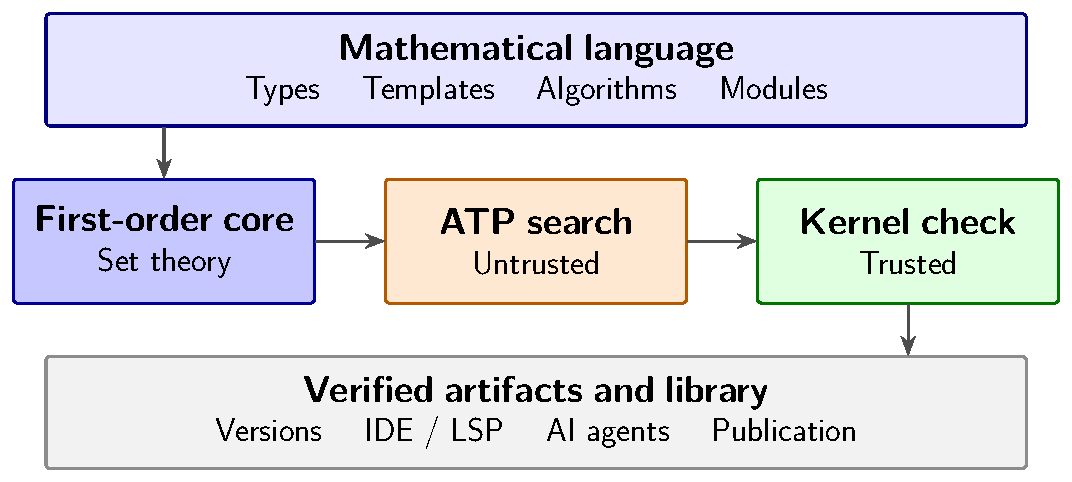
\includegraphics[width=\textwidth,height=0.64\textheight,keepaspectratio]{figures/layer_stack.pdf}
\end{center}
\begin{itemize}
\setlength{\itemsep}{1pt}
\setlength{\parsep}{0pt}
\setlength{\parskip}{0pt}
\item \textcolor{blue!55!black}{\textbf{Support rich mathematical writing with a small first-order foundation and modern development tools.}}
\end{itemize}
\note{
\smallskip
\textbf{Read aloud:}
\begin{itemize}
\setlength{\itemsep}{1pt}
\setlength{\parsep}{0pt}
\setlength{\parskip}{0pt}
\item \textcolor{blue!55!black}{\textbf{Support rich mathematical writing with a small first-order foundation and modern development tools.}}
\end{itemize}
\smallskip
\textbf{Optional notes and sources:}
\begin{itemize}
\setlength{\itemsep}{1pt}
\setlength{\parsep}{0pt}
\setlength{\parskip}{0pt}
\item Elaboration turns mathematical language into a first-order representation. The kernel checks candidate evidence from external ATPs. Checked artifacts and libraries support IDE / LSP, AI, and publication.
\end{itemize}
}
\end{frame}

\section{Part 6. Checking And Automation}
\begin{frame}[fragile,t]{6.1 - Automation: find lemmas and suggest a proof}
\smallskip
\textbf{Isabelle/HOL: Sledgehammer suggests a proof}~\badgeSketch
\begin{lstlisting}[language={},basicstyle=\ttfamily\small]
have "Q a"
  sledgehammer
  by (metis allPQ pa)
\end{lstlisting}
Mizar Evo: request lemma search with \texttt{by atp} (proposed syntax).

\textcolor{blue!55!black}{\textbf{Open goal → library lemma candidates → ATP trials → a \texttt{by} suggestion.}}

\smallskip
\textbf{Request and suggestion (sketch, planned; Pa is the local assumption P(a)):}
\begin{lstlisting}[language={mizar},basicstyle=\ttfamily\small]
thus Q(a) by atp;
:: Suggested proof:
:: library.AllPQ: for x holds P(x) implies Q(x)
thus Q(a) by library.AllPQ, Pa;
\end{lstlisting}
\begin{itemize}
\setlength{\itemsep}{1pt}
\setlength{\parsep}{0pt}
\setlength{\parskip}{0pt}
\item \textcolor{blue!55!black}{\textbf{Reduce manual lemma search. Keep the selected premises explicit in the source.}}
\item Apply the suggestion and verify again. The kernel / SAT checks formula and substitution evidence before acceptance.
\end{itemize}
\note{
\smallskip
\textbf{Read aloud:}
\begin{itemize}
\setlength{\itemsep}{1pt}
\setlength{\parsep}{0pt}
\setlength{\parskip}{0pt}
\item Isabelle/HOL: Sledgehammer suggests a proof.
\item Mizar Evo: request lemma search with \texttt{by atp} (proposed syntax).
\item \textcolor{blue!55!black}{\textbf{Open goal → library lemma candidates → ATP trials → a \texttt{by} suggestion.}}
\item Request and suggestion (sketch, planned; Pa is the local assumption P(a)):
\item \textcolor{blue!55!black}{\textbf{Reduce manual lemma search. Keep the selected premises explicit in the source.}}
\item Apply the suggestion and verify again. The kernel / SAT checks formula and substitution evidence before acceptance.
\end{itemize}
\smallskip
\textbf{Optional notes and sources:}
\begin{itemize}
\setlength{\itemsep}{1pt}
\setlength{\parsep}{0pt}
\setlength{\parskip}{0pt}
\item \texttt{by atp} is proposed syntax for this talk. The specification does not yet define it. Arguments may be added later.
\item Source: specification chapter 22, §22.4.4; chapter 23, §23.5.2. Details and comparison sources: \texttt{draft.ja.md}.
\end{itemize}
}
\end{frame}

\begin{frame}[fragile,t]{6.2 - Using ATPs: search, check, and reuse}
\begin{center}
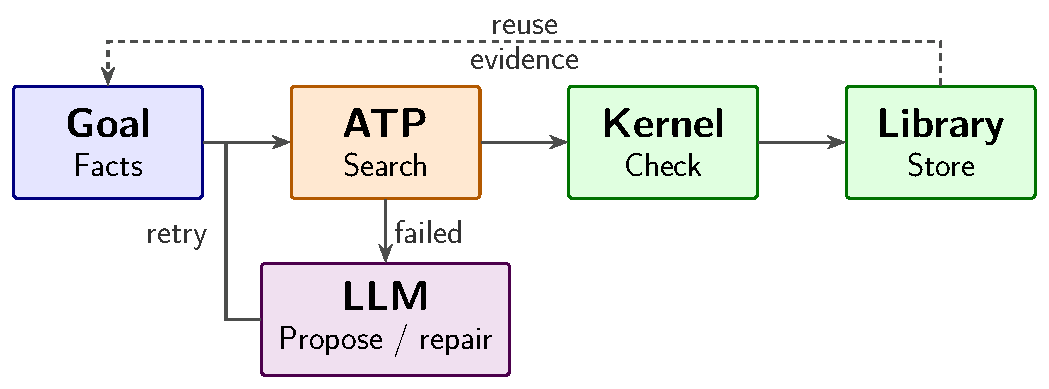
\includegraphics[width=\textwidth,height=0.54\textheight,keepaspectratio]{figures/llm_atp_loop.pdf}
\end{center}
\begin{itemize}
\setlength{\itemsep}{1pt}
\setlength{\parsep}{0pt}
\setlength{\parskip}{0pt}
\item \textcolor{blue!55!black}{\textbf{Goal and premises → ATP search → kernel checking → library storage and reuse.}}
\item If unresolved, revise lemmas or strategy and retry. The figure shows design intent.
\end{itemize}
\note{
\smallskip
\textbf{Read aloud:}
\begin{itemize}
\setlength{\itemsep}{1pt}
\setlength{\parsep}{0pt}
\setlength{\parskip}{0pt}
\item \textcolor{blue!55!black}{\textbf{Goal and premises → ATP search → kernel checking → library storage and reuse.}}
\item If unresolved, revise lemmas or strategy and retry. The figure shows design intent.
\end{itemize}
\smallskip
\textbf{Optional notes and sources:}
\begin{itemize}
\setlength{\itemsep}{1pt}
\setlength{\parsep}{0pt}
\setlength{\parskip}{0pt}
\item LLMs can help suggest and repair proofs. Acceptance depends on evidence checking, explained next.
\item Normal verification uses source citations and local hypotheses. Assistance selects library candidates, tries them, and suggests citations to apply before re-verification. Native-hammer and retry evaluation remains future work.
\item Source: \texttt{doc/spec/en/21.source\_code\_annotation\_and\_atp.md} §21.7.2; \texttt{doc/design/architecture/en/21.ai\_agent\_interface.md}.
\end{itemize}
}
\end{frame}

\begin{frame}[fragile,t]{6.3 - Resolution tree and extracted substitutions}
\smallskip
\textbf{Getting candidate evidence from a resolution log}~\badgeSketch
\begin{center}
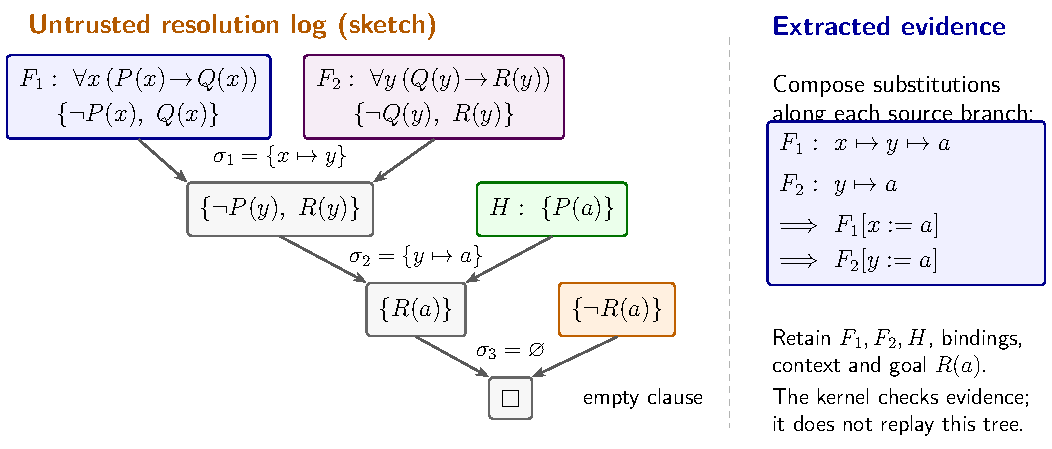
\includegraphics[width=\textwidth,height=0.65\textheight,keepaspectratio]{figures/resolution_evidence.pdf}
\end{center}
\begin{itemize}
\setlength{\itemsep}{1pt}
\setlength{\parsep}{0pt}
\setlength{\parskip}{0pt}
\item \textcolor{blue!55!black}{\textbf{Untrusted extraction: compose to \texttt{x := a} for F1 and \texttt{y := a} for F2.}}
\end{itemize}
\note{
\smallskip
\textbf{Read aloud:}
\begin{itemize}
\setlength{\itemsep}{1pt}
\setlength{\parsep}{0pt}
\setlength{\parskip}{0pt}
\item Getting candidate evidence from a resolution log.
\item \textcolor{blue!55!black}{\textbf{Untrusted extraction: compose to \texttt{x := a} for F1 and \texttt{y := a} for F2.}}
\end{itemize}
\smallskip
\textbf{Optional notes and sources:}
\begin{itemize}
\setlength{\itemsep}{1pt}
\setlength{\parsep}{0pt}
\setlength{\parskip}{0pt}
\item Clause variables x/y have distinct names. Unifying Q gives x:=y; unifying P gives y:=a. Compose them to recover F1[x:=a] and F2[y:=a].
\item This is a proposal for getting candidate evidence from a log. The independent instance finder in architecture 10 is unimplemented (ATP TODO 30). The kernel does not replay each log inference.
\item Source: architecture chapters 08, 10, 15, 16. This is a sketch, not an external-prover execution example.
\end{itemize}
}
\end{frame}

\begin{frame}[fragile,t]{6.4 - From saved evidence to concrete SAT clauses}
\smallskip
\textbf{From evidence checks to SAT-based acceptance}~\badgeSketch
\begin{center}
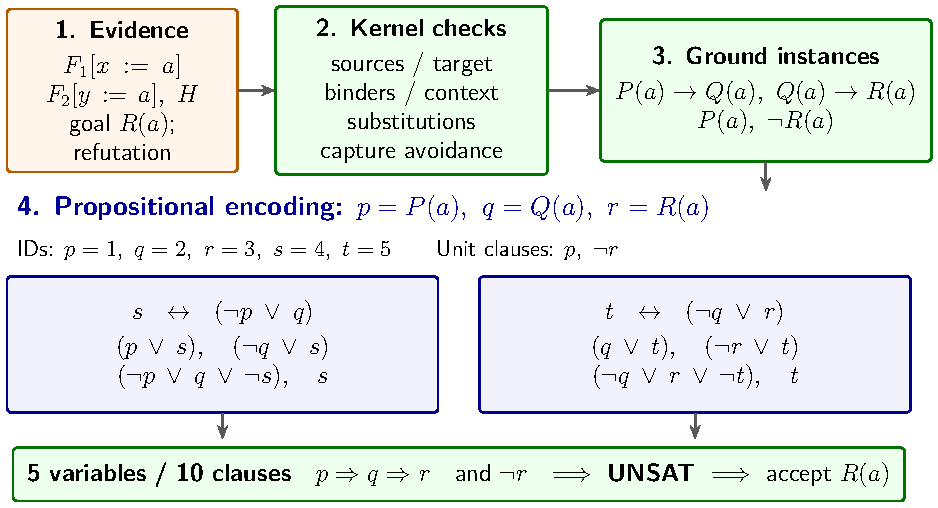
\includegraphics[width=\textwidth,height=0.64\textheight,keepaspectratio]{figures/sat_evidence_check.pdf}
\end{center}
\begin{itemize}
\setlength{\itemsep}{1pt}
\setlength{\parsep}{0pt}
\setlength{\parskip}{0pt}
\item \textcolor{blue!55!black}{\textbf{Check evidence, regenerate CNF, confirm UNSAT with SAT, and accept R(a).}}
\end{itemize}
\note{
\smallskip
\textbf{Read aloud:}
\begin{itemize}
\setlength{\itemsep}{1pt}
\setlength{\parsep}{0pt}
\setlength{\parskip}{0pt}
\item From evidence checks to SAT-based acceptance.
\item \textcolor{blue!55!black}{\textbf{Check evidence, regenerate CNF, confirm UNSAT with SAT, and accept R(a).}}
\end{itemize}
\smallskip
\textbf{Optional notes and sources:}
\begin{itemize}
\setlength{\itemsep}{1pt}
\setlength{\parsep}{0pt}
\setlength{\parskip}{0pt}
\item Save original formulas, composed substitutions, binding context, target VC, and refutation polarity. Regenerate instances and SAT clauses; details in \texttt{draft.ja.md} §6.
\item Each blue box defines implication variable s/t and gives four clauses. With unit clauses p and not r, there are five variables and ten clauses. DIMACS is retained in \texttt{draft.ja.md} §6. This is not an execution dump.
\item The kernel neither searches for substitutions nor replays external resolution steps. Source: architecture chapters 08, 15, 16.
\end{itemize}
}
\end{frame}

\section{Part 7. Status And Roadmap}
\begin{frame}[fragile,t]{7.1 - Implementation status and size}
\textcolor{blue!55!black}{\textbf{Rust product code: 271.1 kLoC; estimated total: 360–540 kLoC (rough estimate).}}

\par\noindent{\footnotesize\bfseries Table 13. Implementation status and code size (kLoC)\par}
\begin{scriptsize}
\setlength{\tabcolsep}{3pt}
\renewcommand{\arraystretch}{1.15}
\begin{tabularx}{\textwidth}{lrr>{\raggedright\arraybackslash}X}
\toprule
\textbf{Area} & \textbf{Now} & \textbf{Est. total} & \textbf{Scope / remaining work} \\
\midrule
lexer / parser / frontend & 34.4 & 36–43 & Syntax, source loading, lexing, parsing connected \\
resolver / checker & 122.9 & 148–193 & Limited source semantics; generalization / services remain \\
Core / VC & 49.7 & 65–95 & IR / proof; limited source to VCs \\
ATP & 9.6 & 16–28 & Encoding / candidates; real backend integration remains \\
kernel & 12.8 & 15–20 & Formula / substitution / provenance checks; includes 1.9 for SAT \\
build / driver / artifact & 41.3 & 56–85 & Cache / shared support; full-pipeline publication not connected \\
LSP & 0.5 & 6–19 & Lifecycle / sync; semantic connections remain \\
MVM / extraction / doc & 0 & 17–57 & Runtime / extraction / docs unimplemented \\
\bottomrule
\end{tabularx}
\end{scriptsize}

\textcolor{blue!55!black}{\textbf{Excluding ATP: kernel + SAT dependencies = 17.6 kLoC.}}

{\footnotesize Core / session counted separately. Excludes dependencies, tests, blank lines, comments. Estimates include current code; rounded.}

{\footnotesize Source: fixed snapshot \texttt{08861708}. Counting and estimate basis: \texttt{draft.ja.md} §7.}

\note{
\smallskip
\textbf{Read aloud:}
\begin{itemize}
\setlength{\itemsep}{1pt}
\setlength{\parsep}{0pt}
\setlength{\parskip}{0pt}
\item \textcolor{blue!55!black}{\textbf{Rust product code: 271.1 kLoC; estimated total: 360–540 kLoC (rough estimate).}}
\item \textcolor{blue!55!black}{\textbf{Excluding ATP: kernel + SAT dependencies = 17.6 kLoC.}}
\item {\footnotesize Core / session counted separately. Excludes dependencies, tests, blank lines, comments. Estimates include current code; rounded.}
\end{itemize}
\smallskip
\textbf{Optional notes and sources:}
\begin{itemize}
\setlength{\itemsep}{1pt}
\setlength{\parsep}{0pt}
\setlength{\parskip}{0pt}
\item 1 kLoC = 1,000 lines. Rough estimates, not yet tested. MML porting is excluded.
\item Kernel 12.751 (SAT encoding / connection: 1.947). SAT dependencies: batsat 0.6.0 + bit-vec 0.5.1 = 4.879; total 17.630 kLoC. Excludes Core / session / shared support; not the full minimum trusted computing base (TCB).
\item Fixed snapshot, limited implementation. Counted October 15, 2026; kernel recount / SAT dependencies, October 16.
\end{itemize}
\begin{itemize}
\setlength{\itemsep}{1pt}
\setlength{\parsep}{0pt}
\setlength{\parskip}{0pt}
\item {\footnotesize Source: fixed snapshot \texttt{08861708}. Counting and estimate basis: \texttt{draft.ja.md} §7.}
\end{itemize}
}
\end{frame}

\begin{frame}[fragile,t]{7.2 - Next steps and summary}
\smallskip
\textbf{Next steps}
\begin{itemize}
\setlength{\itemsep}{1pt}
\setlength{\parsep}{0pt}
\setlength{\parskip}{0pt}
\item \textcolor{blue!55!black}{\textbf{First priority: connect source-to-semantics → VC → evidence → kernel → artifact → build.}}
\item Make algorithm semantics and proof obligations agree; extend the working parts.
\item MVM runtime / extraction: separate work. MML porting is separate from processor completion.
\item Learned premise selection, LLM repair, cryptography, and quantum algorithms are long-term directions.
\end{itemize}
\smallskip
\textbf{Summary}
\begin{itemize}
\setlength{\itemsep}{1pt}
\setlength{\parsep}{0pt}
\setlength{\parskip}{0pt}
\item \textcolor{blue!55!black}{\textbf{Keep FOL, set theory, and mathematical writing; redesign language and tools.}}
\item \textcolor{blue!55!black}{\textbf{Separate ATP search from trusted checking. The specification is still evolving.}}
\item \textcolor{blue!55!black}{\textbf{Please share your ITP needs: notation, proof assistance, development tools.}}
\end{itemize}
\note{
\smallskip
\textbf{Read aloud:}
\begin{itemize}
\setlength{\itemsep}{1pt}
\setlength{\parsep}{0pt}
\setlength{\parskip}{0pt}
\item \textcolor{blue!55!black}{\textbf{First priority: connect source-to-semantics → VC → evidence → kernel → artifact → build.}}
\item Make algorithm semantics and proof obligations agree; extend the working parts.
\item MVM runtime / extraction: separate work. MML porting is separate from processor completion.
\item Learned premise selection, LLM repair, cryptography, and quantum algorithms are long-term directions.
\item \textcolor{blue!55!black}{\textbf{Keep FOL, set theory, and mathematical writing; redesign language and tools.}}
\item \textcolor{blue!55!black}{\textbf{Separate ATP search from trusted checking. The specification is still evolving.}}
\item \textcolor{blue!55!black}{\textbf{Please share your ITP needs: notation, proof assistance, development tools.}}
\end{itemize}
\smallskip
\textbf{Optional notes and sources:}
\begin{itemize}
\setlength{\itemsep}{1pt}
\setlength{\parsep}{0pt}
\setlength{\parskip}{0pt}
\item Source: \texttt{doc/design/todo.md}, integration order and MML-port boundary.
\end{itemize}
}
\end{frame}

\appendix
\section{Backup 1. Template instantiation: one proof, many views}
\begin{frame}[fragile,t]{Backup 1. Template instantiation: one proof, many views}
A generic theorem with a bounded type parameter (specification example, proof omitted):

\begin{lstlisting}[language={mizar},basicstyle=\ttfamily\footnotesize]
definition
  let T be type extends commutative associative unital Magma;
  theorem PermProduct[T]:
    for s being FinSequence of T,
        p being Permutation of dom s
    holds Product[T](s) = Product[T](s * p)
  proof ... end;
end;
\end{lstlisting}
\smallskip
\textbf{Instances}~\badgeSpec~{\footnotesize(assuming the required registrations)}
\begin{lstlisting}[language={mizar},basicstyle=\ttfamily\small]
PermProduct[commutative associative unital AddMagma]
PermProduct[commutative associative unital MulMagma]
let R be commutative Ring;  PermProduct[R qua AddMagma]  :: additive view
\end{lstlisting}
\begin{itemize}
\setlength{\itemsep}{1pt}
\setlength{\parsep}{0pt}
\setlength{\parskip}{0pt}
\item A ring has two inheritance paths to Magma. The view selected by \texttt{qua} determines the notation.
\end{itemize}
\note{
\smallskip
\textbf{Read aloud:}
\begin{itemize}
\setlength{\itemsep}{1pt}
\setlength{\parsep}{0pt}
\setlength{\parskip}{0pt}
\item A generic theorem with a bounded type parameter.
\item Instances.
\item A ring has two inheritance paths to Magma. The view selected by \texttt{qua} determines the notation.
\end{itemize}
\smallskip
\textbf{Optional notes and sources:}
\begin{itemize}
\setlength{\itemsep}{1pt}
\setlength{\parsep}{0pt}
\setlength{\parskip}{0pt}
\item Source: \texttt{doc/spec/en/18.templates.md}, section 18.2.2.
\end{itemize}
}
\end{frame}

\section{Backup 2. Incremental verification}
\begin{frame}[fragile,t]{Backup 2. Incremental verification}
\begin{center}
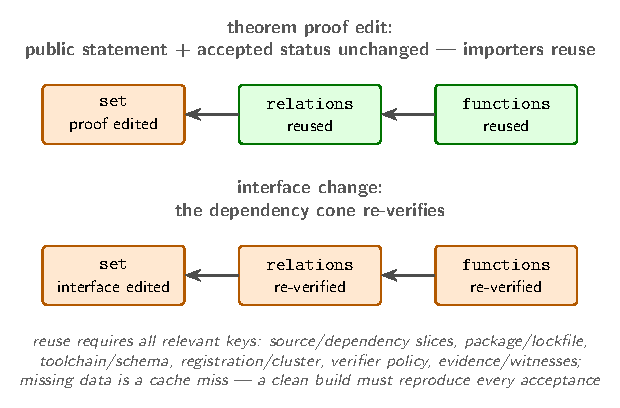
\includegraphics[width=\textwidth,height=0.52\textheight,keepaspectratio]{../2026-09-bialystok/figures/fingerprint_graph.pdf}
\end{center}
\begin{itemize}
\setlength{\itemsep}{1pt}
\setlength{\parsep}{0pt}
\setlength{\parskip}{0pt}
\item A proof-body edit needs no rebuild of other modules if the public claim and acceptance status stay unchanged. An interface change rechecks all direct and indirect dependents.
\item Reuse needs exact matches for all relevant cache keys. Missing data means a miss. A clean build must reproduce every accepted result; reuse alone does not prove correctness.
\end{itemize}
\note{
\smallskip
\textbf{Read aloud:}
\begin{itemize}
\setlength{\itemsep}{1pt}
\setlength{\parsep}{0pt}
\setlength{\parskip}{0pt}
\item A proof-body edit needs no rebuild of other modules if the public claim and acceptance status stay unchanged. An interface change rechecks all direct and indirect dependents.
\item Reuse needs exact matches for all relevant cache keys. Missing data means a miss. A clean build must reproduce every accepted result; reuse alone does not prove correctness.
\end{itemize}
\smallskip
\textbf{Optional notes and sources:}
\begin{itemize}
\setlength{\itemsep}{1pt}
\setlength{\parsep}{0pt}
\setlength{\parskip}{0pt}
\item Source: \texttt{doc/design/architecture/en/11.artifact\_and\_incremental\_build.md}, \texttt{18.dependency\_fingerprint.md}; Bia\l{}ystok deck, Story 5.
\end{itemize}
}
\end{frame}

\section{Backup 3. Package manifest}
\begin{frame}[fragile,t]{Backup 3. Package manifest}
\smallskip
\textbf{Mizar Evo}~\badgeSpec
\begin{lstlisting}[language={toml},basicstyle=\ttfamily\footnotesize]
[package]
name    = "algebra"
version = "2.3.1"
edition = "2025"

[dependencies]
mml_core = "^1.0"
topology = { version = "^0.9", features = ["metric"] }
\end{lstlisting}
\begin{itemize}
\setlength{\itemsep}{1pt}
\setlength{\parsep}{0pt}
\setlength{\parskip}{0pt}
\item Reproducible builds need fixed sources, lockfile, toolchain, checker configuration, and deterministic ATP evidence.
\item Versions let authors reuse articles without manual copies between libraries. One module can collect a field's public items into a single import.
\end{itemize}
Source: \texttt{doc/spec/en/23.package\_management\_and\_build\_system.md}; Bia\l{}ystok deck, Story 1.

\note{
\smallskip
\textbf{Read aloud:}
\begin{itemize}
\setlength{\itemsep}{1pt}
\setlength{\parsep}{0pt}
\setlength{\parskip}{0pt}
\item Reproducible builds need fixed sources, lockfile, toolchain, checker configuration, and deterministic ATP evidence.
\item Versions let authors reuse articles without manual copies between libraries. One module can collect a field's public items into a single import.
\end{itemize}
\smallskip
\textbf{Optional notes and sources:}
\begin{itemize}
\setlength{\itemsep}{1pt}
\setlength{\parsep}{0pt}
\setlength{\parskip}{0pt}
\item Source: \texttt{doc/spec/en/23.package\_management\_and\_build\_system.md}; Bia\l{}ystok deck, Story 1.
\end{itemize}
}
\end{frame}

\section{Backup 4. Comparing evaluation conditions}
\begin{frame}[fragile,t]{Backup 4. Comparing evaluation conditions}
\par\noindent{\footnotesize\bfseries Table 14. MizAR 60 and Sledgehammer evaluation conditions\par}
\begin{scriptsize}
\setlength{\tabcolsep}{3pt}
\renewcommand{\arraystretch}{1.15}
\begin{tabularx}{\textwidth}{l>{\raggedright\arraybackslash}X>{\raggedright\arraybackslash}X}
\toprule
\textbf{} & \textbf{MizAR 60 (ITP 2023)} & \textbf{Sledgehammer / AFP (ITP 2022)} \\
\midrule
Reported success & 58.4\% (1,690 / 2,896) & 68.8\% (3,440 / 5,000) \\
Evaluation set & MML 1147 theorems / lemmas; 2,896 holdout problems out of 57,897 & 5,000 local goals from 50 AFP entries \\
Premise selection & Learned selection from the whole library & MePo; baseline 512 facts, varied by configuration \\
Time budget & Portfolio total: 420 CPU seconds & Greedy 16 configurations × 30 CPU seconds = 480 CPU seconds \\
Success criterion & ATP proof found (hammering mode) & External-prover proof found; Isabelle reconstruction excluded \\
\bottomrule
\end{tabularx}
\end{scriptsize}

\begin{itemize}
\setlength{\itemsep}{1pt}
\setlength{\parsep}{0pt}
\setlength{\parskip}{0pt}
\item \textcolor{blue!55!black}{\textbf{Different targets, premise selection, time budgets, and configuration choices. Success rates alone cannot rank the designs.}}
\end{itemize}
\note{
\smallskip
\textbf{Read aloud:}
\begin{itemize}
\setlength{\itemsep}{1pt}
\setlength{\parsep}{0pt}
\setlength{\parskip}{0pt}
\item \textcolor{blue!55!black}{\textbf{Different targets, premise selection, time budgets, and configuration choices. Success rates alone cannot rank the designs.}}
\end{itemize}
\smallskip
\textbf{Optional notes and sources:}
\begin{itemize}
\setlength{\itemsep}{1pt}
\setlength{\parsep}{0pt}
\setlength{\parskip}{0pt}
\item A hammer sends goals to automated provers. Premises are facts the prover may use.
\item Source: Jakubův et al. 2023, §6.2, 6.5; Desharnais et al. 2022, §5, 5.6, Table 10. The greedy configurations were selected after testing on the same evaluation set.
\item Publication and experiment dates differ: main MizAR experiments, 2020–2021; AFP evaluation, Isabelle from January 2022 and AFP from December 2021.
\item MizAR's 75\% figure uses library premises selected by a human or a machine. Keep it for questions.
\end{itemize}
}
\end{frame}

\section{Backup 5. HOL encoding and reconstruction}
\begin{frame}[fragile,t]{Backup 5. HOL encoding and reconstruction}
\smallskip
\textbf{Outline of encoding steps}~\badgeSketch
\begin{lstlisting}[language={},basicstyle=\ttfamily\footnotesize]
F X                   ->  app(F, X)
(%x. t) ...           ->  fresh constant + defining axioms   (lambda lifting)
polymorphic types     ->  type guards or type tags
Boolean-valued terms  ->  extra encoding
\end{lstlisting}
\begin{itemize}
\setlength{\itemsep}{1pt}
\setlength{\parsep}{0pt}
\setlength{\parskip}{0pt}
\item \textcolor{blue!55!black}{\textbf{Use \texttt{app} for function-variable application. Encode lambdas with lambda lifting or combinators, and types with guards or tags.}}
\item \textcolor{blue!55!black}{\textbf{Reconstruct the ATP proof inside Isabelle: \texttt{metis}, \texttt{smt} replay, or generated Isar text.}}
\item These techniques connect higher-order ITPs to first-order ATPs.
\item This explains the connection, not a measured performance advantage.
\end{itemize}
\note{
\smallskip
\textbf{Read aloud:}
\begin{itemize}
\setlength{\itemsep}{1pt}
\setlength{\parsep}{0pt}
\setlength{\parskip}{0pt}
\item Outline of encoding steps.
\item \textcolor{blue!55!black}{\textbf{Use \texttt{app} for function-variable application. Encode lambdas with lambda lifting or combinators, and types with guards or tags.}}
\item \textcolor{blue!55!black}{\textbf{Reconstruct the ATP proof inside Isabelle: \texttt{metis}, \texttt{smt} replay, or generated Isar text.}}
\item These techniques connect higher-order ITPs to first-order ATPs.
\item This explains the connection, not a measured performance advantage.
\end{itemize}
\smallskip
\textbf{Optional notes and sources:}
\begin{itemize}
\setlength{\itemsep}{1pt}
\setlength{\parsep}{0pt}
\setlength{\parskip}{0pt}
\item Source: Meng and Paulson 2008 (higher-order to first-order clauses); Blanchette, Böhme, Popescu, Smallbone 2016 (type encoding); Blanchette, Kaliszyk, Paulson, Urban 2016 (survey); Schurr, Fleury, Desharnais 2021 (reconstruction).
\item The actual Sledgehammer encoding depends on prover and options. This is an outline.
\end{itemize}
}
\end{frame}

\end{document}
